\section{Auswertung}
%zuerst !alle! errechneten werte entweder in ganzen s�tzen aufz�hlen, oder in tabellen (�bersichtlicher) dargestellen, sowie auf die verwendeten formeln verweisen (die referenzierung der formel kann in der �berschrift stehen)
%kurz erw�hnen (vor der tabelle), warum wir das ganze ausrechnen bzw. was wir dort ausrechnen
%danach histogramme und plots erstellen, wobei wenn m�glich funktionen durch die plots gelegt werden (zur not k�nnen auch splines benutzt werden, was aber angegeben werden muss)
%bei fits immer die funktion und das reduzierte chiquadrat mit angegeben, wobei auf verst�ndlichkeit beim entziffern der zehnerpotenzen geachtet werden muss z.b. f(x)=(wert+-fehler)\cdot10^{irgendeine zahl}\cdot x + (wert+-fehler)\cdot10^{irgendeine zahl}
%bei jedem fit erkl�ren, nach welchem zusammenhang gefittet wurde und warum!
%bei plots darauf achten, dass die achsenbeschriftung (auch die tics) die richtige gr��e haben und die legende im plot nicht die messwerte verdeckt
%kurz die aufgabenstellung abgehandeln
Die gemessenen Daten werden in Abb. \ref{fig:Kanal_Eintr�ge_Fehler_Plot} dargestellt.
\begin{figure}[H]
\centering
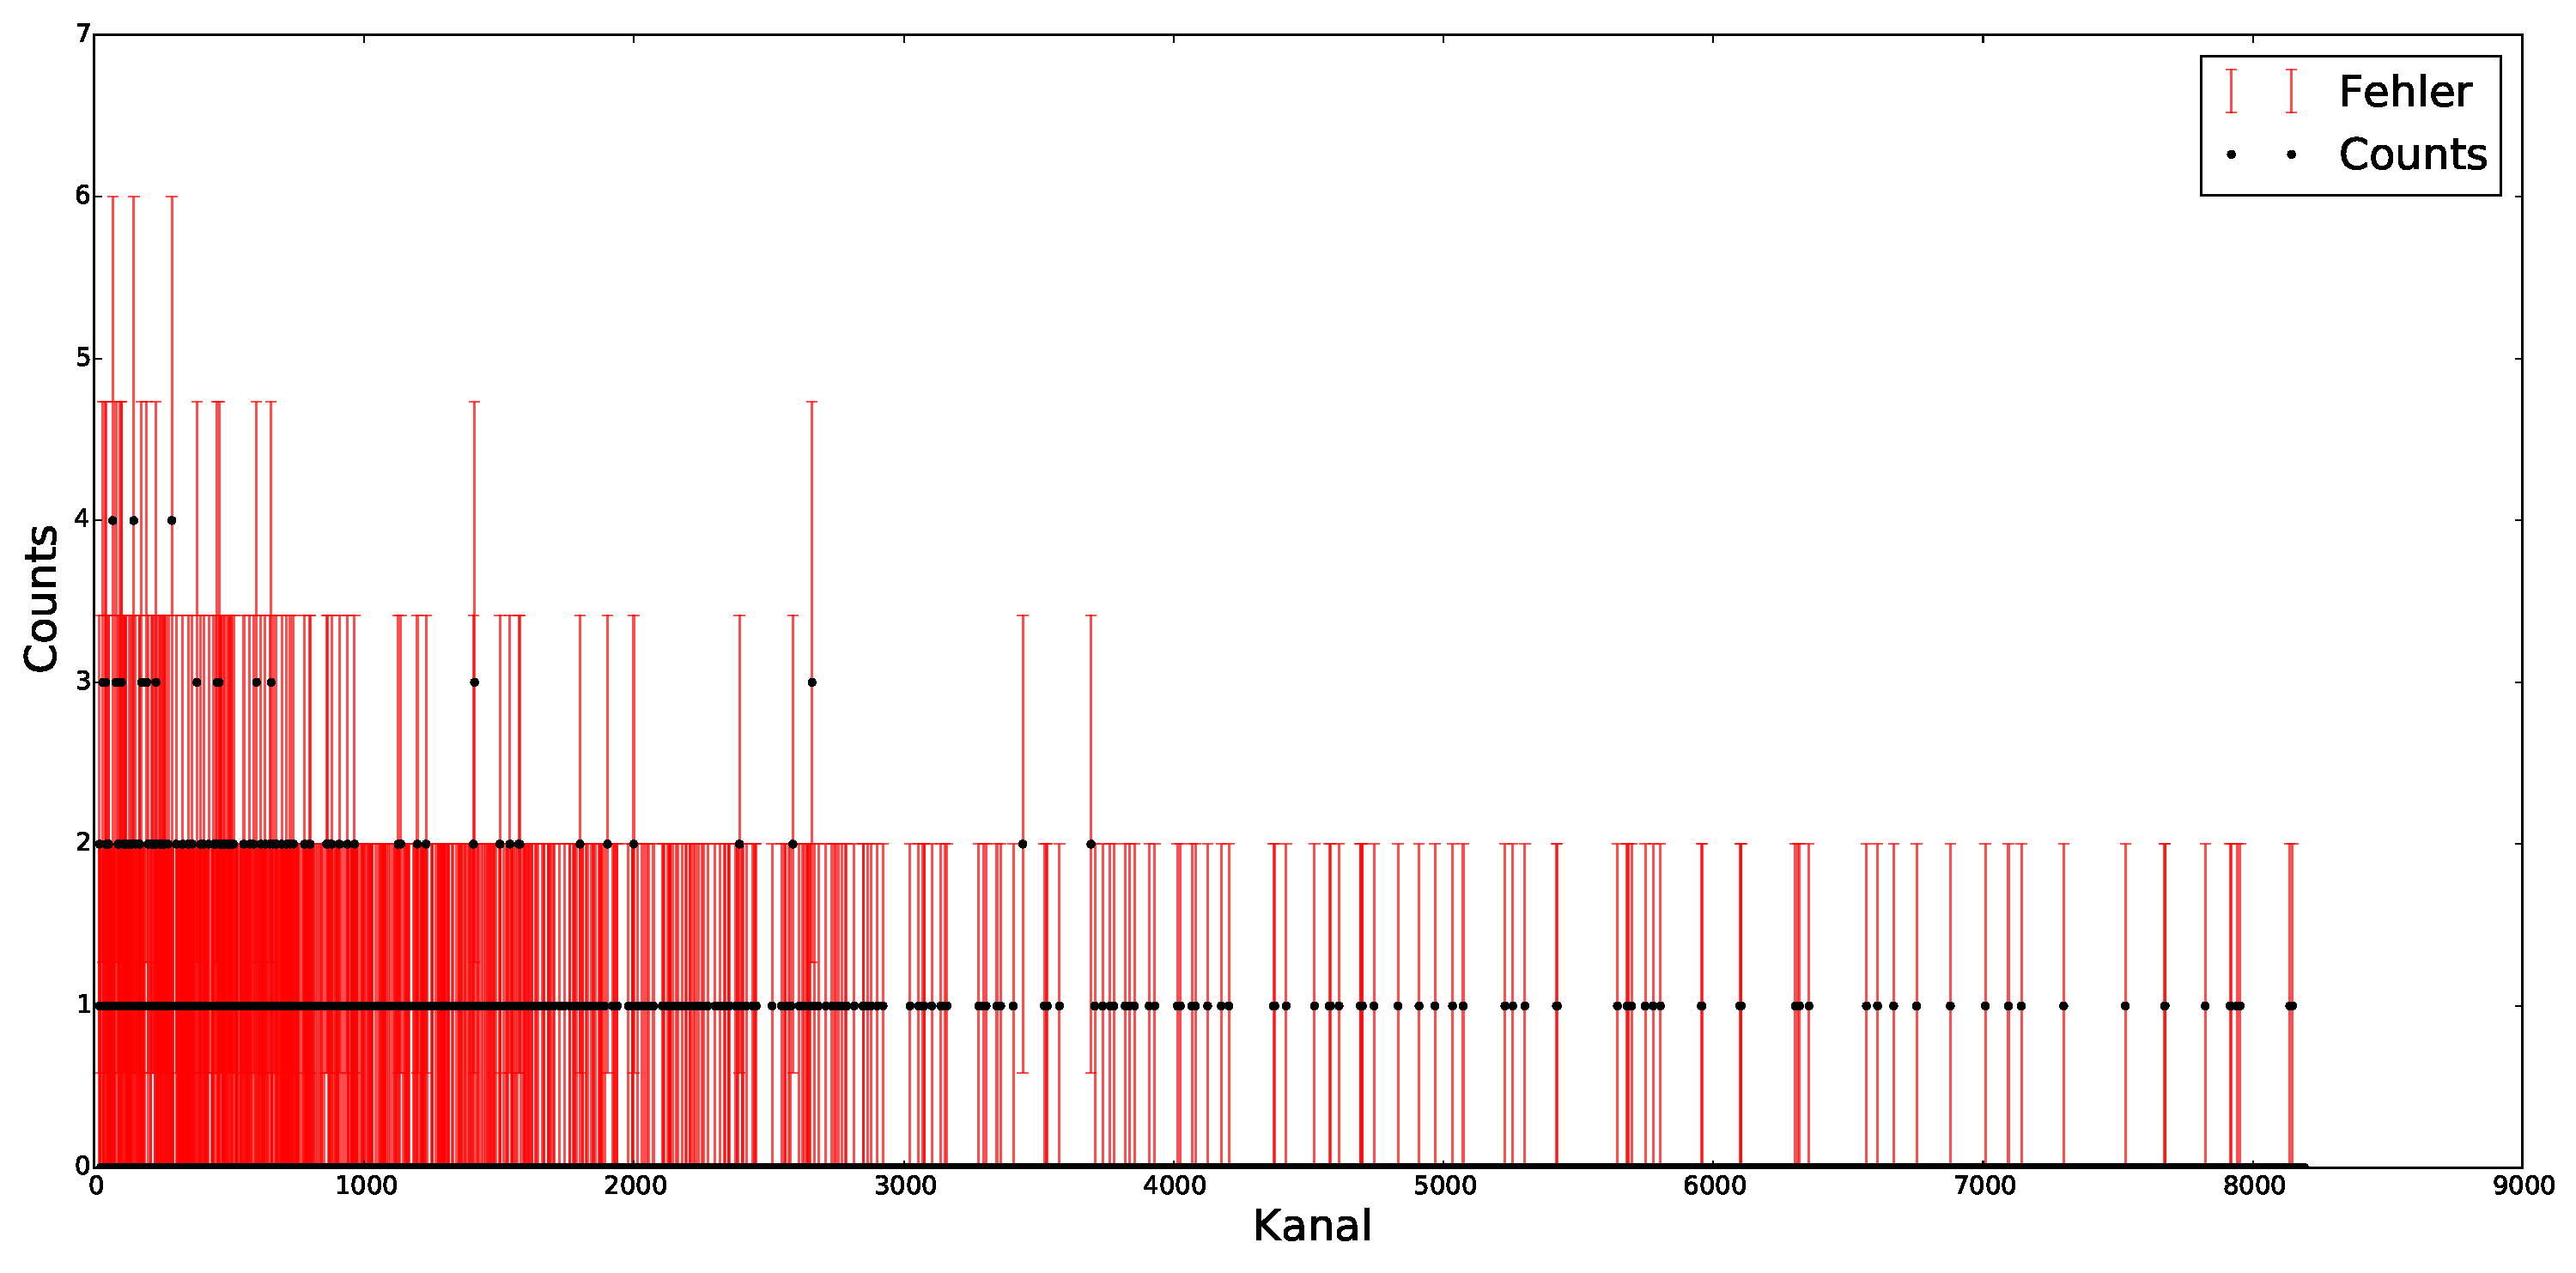
\includegraphics[scale = 0.35]{Kanal_Eintraege_Fehler_Plot}
\caption{Plot der Eintr�ge gegen die Kan�le ab Channel 18}
\label{fig:Kanal_Eintr�ge_Fehler_Plot}
\end{figure}
Die ersten 17 Kan�le sind dabei wegen starkem Rauschen unbrauchbar und wurden deshalb weggelassen. Die mittlere Lebensdauer soll nun mit der Maximum Likelihood Methode bestimmt werden. Daf�r wurde ein Programm in Python geschrieben, welches $\tau$ (= mittlere Lebensdauer) iterativ mittels Formel \ref{eqn:tau_rek} rekursiv bestimmt. Als Startwert wird der Mittelwert (Formel \ref{eqn:startwert}) verwendet. Der Python-Code kann im Anhang nachvollzogen werden. Die Iteration wurde f�r beide Kanal-Zeit-Eichungen durchgef�hrt und wurde nach Konvergenz in der 24. Nachkommastelle abgebrochen. Die Ergebnisse sind in Tabelle \ref{tab:maximum_likelihood_iteration} dargestellt.
\begin{table}[H]
\centering
\caption{Iteration f�r $\hat{\tau}$}
\begin{tabular}{|c|c|c|c|c|}
\hline $f(k)$ Kanal-Zeit & $\tau_0/\mu s$ & Iterationsschritte & $\hat{\tau}/\mu s$ & $\Delta\hat{\tau}/\mu s$ \\ 
\hline $A*k+B$ & 2.93 & 16 & 2.98 & 0.15 \\ 
\hline $A*k$ & 2.85 & 15 & 2.89 & 0.15 \\ 
\hline 
\end{tabular} 
\label{tab:maximum_likelihood_iteration}
\end{table}
Man sieht sofort, dass die Iteration nach wenigen Schritten konvergiert, wobei die bestimmten Lebensdauern im Vergleich zum Literaturwert $\tau_{lit} = \SI{2,1969811(22)}{$\mu$s}$ (vgl. \cite{wiki_myon}) zu gro� sind. Aufgrund der geringen statistischen Fehler auf die Zeiten $t_k$ und $T$, wurden diese nicht in die Berechnung des Gesamtfehlers f�r $\hat{\tau}$ mit einbezogen.